\documentclass[border=10pt]{standalone}
\usepackage[T1]{fontenc}
\usepackage[utf8]{inputenc}
\usepackage[scaled=0.95]{helvet}
\renewcommand{\familydefault}{\sfdefault}
\usepackage{xcolor}
\definecolor{terracotta}{HTML}{C2410C}
\definecolor{sarcelle}{HTML}{0F766E}
\definecolor{violet}{HTML}{7C3AED}
\definecolor{encre}{HTML}{1C1917}
\definecolor{gris}{HTML}{78716C}
\definecolor{grisclair}{HTML}{F5F5F4}
\definecolor{ambre}{HTML}{B45309}
\usepackage{tikz}
\usetikzlibrary{positioning,arrows.meta,fit,backgrounds,calc}
\tikzset{
  boite/.style={draw=#1,fill=#1!7,rounded corners=4pt,align=center,minimum height=1cm,text width=2.9cm,line width=0.8pt,text=encre},
  boite/.default=gris,
  titre/.style={font=\small\bfseries,text=#1},
  fleche/.style={-{Stealth[length=2.6mm]},line width=0.8pt,color=gris},
}
\color{encre}

\usepackage{pgfplots}
\pgfplotsset{compat=1.17}
\usepackage{sansmath}
\begin{document}\sansmath
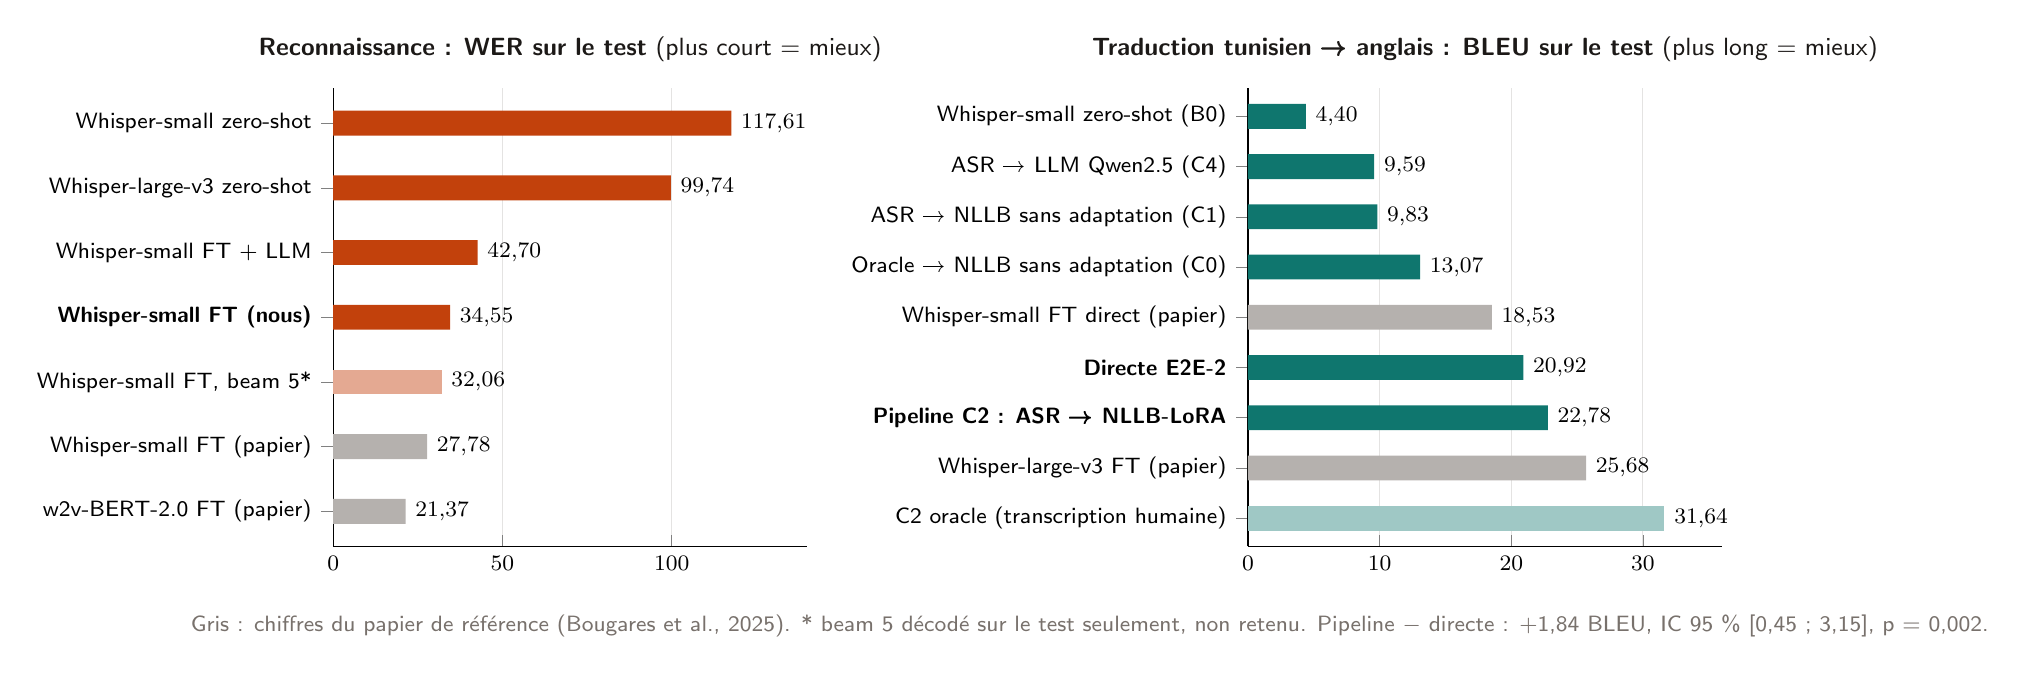
\begin{tikzpicture}[font=\small]
\begin{axis}[name=asr,
  title={\textbf{Reconnaissance : WER sur le test} (plus court = mieux)}, title style={text=encre},
  xbar, width=7.6cm, height=7.4cm, xmin=0, xmax=140,
  symbolic y coords={P-w2v,P-small,O-beam,O-ft,O-llm,O-large,O-small},
  ytick={P-w2v,P-small,O-beam,O-ft,O-llm,O-large,O-small},
  yticklabels={{w2v-BERT-2.0 FT (papier)},{Whisper-small FT (papier)},{Whisper-small FT, beam 5*},{\textbf{Whisper-small FT (nous)}},{Whisper-small FT + LLM},{Whisper-large-v3 zero-shot},{Whisper-small zero-shot}},
  yticklabel style={font=\footnotesize,align=right},
  xticklabel style={font=\footnotesize},
  bar width=9pt, bar shift=0pt, enlarge y limits=0.09,
  nodes near coords, nodes near coords style={font=\footnotesize,/pgf/number format/.cd,fixed,fixed zerofill,precision=2,use comma},
  axis x line*=bottom, axis y line*=left, xmajorgrids, grid style={gris!20},
  every axis plot/.append style={draw=none}]
\addplot[fill=terracotta] coordinates {(117.61,O-small) (99.74,O-large) (42.70,O-llm) (34.55,O-ft)};
\addplot[fill=terracotta!45] coordinates {(32.06,O-beam)};
\addplot[fill=gris!55] coordinates {(27.78,P-small) (21.37,P-w2v)};
\end{axis}
\begin{axis}[at={($(asr.east)+(5.6cm,0)$)},anchor=west,
  title={\textbf{Traduction tunisien → anglais : BLEU sur le test} (plus long = mieux)}, title style={text=encre},
  xbar, width=7.6cm, height=7.4cm, xmin=0, xmax=36,
  symbolic y coords={orac,pbest,c2,e2e,psmall,c0,c1,c4,b0},
  ytick={orac,pbest,c2,e2e,psmall,c0,c1,c4,b0},
  yticklabels={{C2 oracle (transcription humaine)},{Whisper-large-v3 FT (papier)},{\textbf{Pipeline C2 : ASR → NLLB-LoRA}},{\textbf{Directe E2E-2}},{Whisper-small FT direct (papier)},{Oracle → NLLB sans adaptation (C0)},{ASR → NLLB sans adaptation (C1)},{ASR → LLM Qwen2.5 (C4)},{Whisper-small zero-shot (B0)}},
  yticklabel style={font=\footnotesize,align=right},
  xticklabel style={font=\footnotesize},
  bar width=9pt, bar shift=0pt, enlarge y limits=0.07,
  nodes near coords, nodes near coords style={font=\footnotesize,/pgf/number format/.cd,fixed,fixed zerofill,precision=2,use comma},
  axis x line*=bottom, axis y line*=left, xmajorgrids, grid style={gris!20},
  every axis plot/.append style={draw=none}]
\addplot[fill=sarcelle] coordinates {(4.40,b0) (9.59,c4) (9.83,c1) (13.07,c0) (20.92,e2e) (22.78,c2)};
\addplot[fill=sarcelle!40] coordinates {(31.64,orac)};
\addplot[fill=gris!55] coordinates {(18.53,psmall) (25.68,pbest)};
\end{axis}
\node[font=\footnotesize,text=gris,anchor=north] at ($(asr.south)!0.5!(asr.south)+(6.6cm,-0.75cm)$) {Gris : chiffres du papier de référence (Bougares et al., 2025). * beam 5 décodé sur le test seulement, non retenu. Pipeline $-$ directe : +1,84 BLEU, IC 95 \% [0,45 ; 3,15], p = 0,002.};
\end{tikzpicture}
\end{document}
